\chapter{Praktická aplikace}
Vzhled a ovládání celé aplikace je velmi jednoduché a intuitivní. Na úvodní stránce je přehled všech zařízení zapojených do sítě včetně jejich stavu. Vedle názvu zařízení je vidět, jestli je online, či nikoliv. Pod názvem je vidět aktuální přijatá informace v číselné podobě. Následuje seznam připojených a připojitelných zařízení. Jedním kliknutím je možné propojit jakékoliv koncentrátory. V tu chvíli začne server přeposílat příchozí data na všechna připojená zařízení. Daným zařízením posílá pouze ty informace, které jim posílat má. To je dáno právě tím, jaké zařízení je propojeno s kterým. Počet připojitelných zařízení není nijak omezen. Toto je velká výhoda celého projektu. Není totiž vázán na fyzická spojení a příchozí data je tak možné poslat všem v síti bez dalších technických komplikací. Ačkoliv Redis \cite{redis} není relační databáze, tak se v ní mimo jiné uchovávají hlavně relace. Relační databáze nebyla zvolena hlavně proto, že nedosahují takových výkonů, jako právě Redis.

\begin{figure}[H]
    \centering
	\makebox[\textwidth]{\includegraphics[width=\textwidth]{img/speedy1.png}}
	\caption{Úvodní stránka aplikace - přehled připojených zařízení}
	\label{fig:speedy1}
\end{figure}

Detail konkrétního zařízení poskytuje podobný pohled, navíc však ukazuje dodatečné informace jako jsou například IP adresy, nebo čas posledního ohlášení. Kromě samotné vizualizace historie příchozích dat je možné nastavit charakter dat odchozích. To znamená, že když bude připojeno další zařízení, nebudou se data rovnou přeposílat, ale najde se příslušná hodnota podle zvolené funkce a tato hodnota se pošle. Ve výchozím stavu se vše chová lineárně, tzn. jaká informace přijde, taková se přeposílá. Je však možné zvolit exponenciální viz rovnice \ref{eq:exp}, logaritmický (\ref{eq:log}), nebo vlnitý charakter (\ref{eq:vlna}). Tyto funkce jsou výsledkem aproximace ručně zvolených funkcí. Byl kladen důraz na to, aby funkce v celém svém rozsahu měly nějakou rozumnou hodnotu. Zároveň jsou v projektu zařazeny i zdánlivě nesmyslné funkce (např. \ref{eq:vlna}), ty jsou zde pro ukázání možností systému. Poslední variantou je boolean závislost, kdy do hodnoty 512 včetně je výstupem 0, jinak maximální hodnota. Lze ji tedy definovat jako upravenou Heavisideovu funkci viz \ref{eq:bool}.

\begin{equation}
	y_{\_exp} = 1.80753 \cdot 1.00625^x
	\label{eq:exp}
\end{equation}

\begin{equation}
	y_{\_log} = -1053.96 + 289.931 \cdot ln(x)
	\label{eq:log}
\end{equation}

\begin{multline}
	y_{\_vlna} = -3.23206 \cdot 10^{-8} \cdot x^4 + 0.000068 \cdot x^3 - 0.044362 \cdot x^2 + \\
				+9.59513 \cdot x - 47.9076
	\label{eq:vlna}
\end{multline}

\begin{equation}
	y_{\_bool} = \left\{
		\begin{matrix}
			0 & \mbox{ pro }x \leq 512 \\
			1023 & \mbox{ pro }x > 512
		\end{matrix}
	\right.
	\label{eq:bool}
\end{equation}

Tyto funkce jsou naprogramovány ve složce \texttt{api/services} v souboru \texttt{FunctionsService.js}. Ukázková implementace logaritmické funkce vypadá takto:

\begin{minted}[linenos,breaklines]{js}
logarithmic: function (device, after_callback) {
  RedisService.del(device + ':table');
  for (var iterator = 0; iterator <= 1023; iterator++) {
    var entry = -1053.96 + (289.931 * (Math.log(iterator) / Math.log(Math.exp(1))));
    entry = entry <= 0 ? 0 : entry;
    entry = entry >= 1023 ? 1023 : entry;
    RedisService.hmset(device + ':table', iterator, Math.round(entry));
  }
  after_callback();
},
\end{minted}

Funkce tedy nejdříve maže předchozí převodní tabulku a následně ukládá nové vypočtené hodnoty. Pomocí ternárního operátoru \cite{ternar} jsou pak implementovány omezovače hodnot.

\begin{figure}[h]
	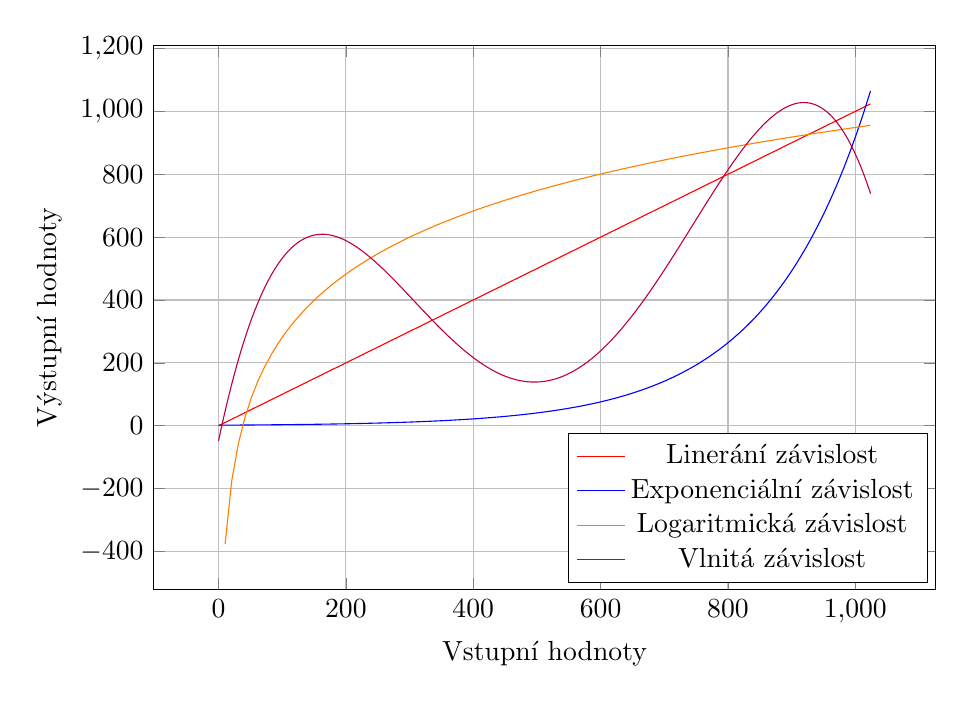
\begin{tikzpicture}
		\begin{axis}[width=0.95\textwidth,height=0.7\textwidth,xlabel={Vstupní hodnoty},ylabel={Výstupní hodnoty},legend style={at={(0.99,0.15)},anchor=east},grid=major]
			\addplot[red,domain=0:1024,samples=10]{x};
			\addlegendentry{Linerání závislost}
			\addplot[blue,domain=0:1024,samples=100]{1.80753*(1.00625^x)};
			\addlegendentry{Exponenciální závislost}
			\addplot[orange,domain=0:1024,samples=100]{-1053.96+(289.931*(ln(x)))};
			\addlegendentry{Logaritmická závislost}
			\addplot[purple,domain=0:1024,samples=200]{(-0.0000000323206*x^4)+(0.000068*x^3)+(-0.044362*x^2)+(9.59513*x)-47.9076};
			\addlegendentry{Vlnitá závislost}
	    \end{axis}
	\end{tikzpicture}
	\caption{Převodní funkce vstupních hodnot}
\end{figure}

Cílem této ukázky je ještě jednou znázornit, že celý systém pracuje na základě přeposílání jasně daných informací, které jsou realizovány pomocí jednoduchých čísel. Je tak možné provádět jakékoliv matematické operace bez nutnosti znalosti významu této informace. Tento přístup však není i\-de\-ál\-ní. V první řadě se až postupem času ukázalo, že rozsah 1024 hodnot je pro určité případy malý. To se projevuje u rychlých výstupů (například u diody). Jde totiž o to, že v určité hodnotě má výstup na který je připojená dioda jedno efektivní napětí a o jeden krok dále je toto napětí o mnoho větší, protože takový je vypočtený výstup z převodní funkce (hodnota $300 \Rightarrow 1,3\,V$ ale $301 \Rightarrow 1,5\,V$). I při nejpomalejších změnách hodnot jsou tyto kroky rozpoznatelné, rychlost zde nehraje hlavní roli. Jedná se o nepatrné změny, jsou však postřehnutelné. A to tím více, čím je nárůst hodnot strmější, tedy jak moc velká chyba vzniká v převodní tabulce. Jedno z možných řešení je zjemnění celého rozsahu, nebo neumožnění velkých skokových změn například pomocí některého z druhů klouzavého průměru. Je však zapotřebí myslet na to, že i tyto úpravy mají své nevýhody. V prvním případě množství hodnot a stále větší kmitání kolem jedné hodnoty, v druhém případě zpomalení systému.

Jedním z možných vylepšení je tak dvojité chování serveru. Ten by totiž mohl přijímat jak převedené hodnoty, tak obecné hodnoty z čidla. Server by jim sice nemohl rozumět (pokud by neměl sám implementovanou převodní tabulku), ale mohl by informaci přeposílat dále do sítě. Tato funkce v současné době není implementovaná a to hlavně z toho důvodu, že je náročné tyto informace nějakým způsobem využívat a skladovat v databázi, protože se jedná o velmi konkrétní problémy vázané na konkrétního výrobce zařízení, nebo čidla. Oproti tomu číselná interpretace hodnot dobře ukazuje, co je v této síti možné vytvořit.

\begin{figure}[h]
    \centering
	\makebox[\textwidth]{\includegraphics[width=\textwidth]{img/speedy2.png}}
	\caption{Detailní pohled na připojené zařízení}
	\label{fig:speedy2}
\end{figure}

Vzhledem ke svým vlastnostem je možné tuto síť použít jako domovní síť pro ovládání běžných prvků, což byl prvotní účel. Z hlediska technologie však tato síť není limitována pouze na ovládání elektroinstalace, ale je možné ji využít pro jakoukoliv senzorickou síť pro sběr dat a zároveň ovládání koncových členů. Její rozumné využití by bylo však tam, kde se bude struktura sítě často měnit, nebo zařízení přesouvat.

\chapter{Rozšíření stávajícího řešení}
Stávající řešení je plně funkční a splňuje veškeré požadavky v zadání. Jedná se však pouze o základ na kterém lze stavět systém, který by bylo možné použít v reálných budovách. Prvně je totiž zapotřebí tuto síť zabezpečit. To se týká zejména okamžiku, kdy by síť začala komunikovat přes Wi-Fi \index{Wi-Fi} (nebo jinou bezdrátovou technologii), ale platí to stejně i pro metalické vedení. Nesmí být možné, aby mohl kdokoliv ovlivňovat chování sítě, pokud k tomu není oprávněn.

Jak bylo již řečeno, samotná myšlenka není nijak limitována na přenos informace pomocí vodičů a je možné použít bezdrátovou komunikaci. Jednou ze zajímavých způsobů bezdrátové komunikace, ačkoliv také možná poněkud futuristickým, je Li-Fi \cite{lifi}. \index{Li-Fi} Tuto komunikaci poprvé představil prof. Harald Haas v roce 2011 v Edinburghu při vystoupení na konferenci TEDGlobal \cite{ted}. Jedná se o přenos informace pomocí viditelného světla. Tento přístup má celou řadu výhod. Kromě kapacity a efektivnosti stojí za zmínku hlavně fakt, že každý v budovách svítí a je tedy pro tento přenos informací vlastně připraven. V neposlední řadě se jedná o bezpečný přenos a to jak z hlediska lidského zdraví, tak i z hlediska různých nežádoucích odposlechů, protože se informace šíří pouze tam, kam dané světlo svítí (nikoliv např. skrz zeď). Síla a dosah signálu jsou tedy doslova vidět.

Dalším důležitým prvkem je implementace IPv6. \index{IPv6} Tyto adresy je možné využívat již od verze 1.4.x LwIP odděleně. V pozdějších verzích by mělo být možné použití IPv4 a IPV6 současně. \index{LwIP} V současné chvíli je totiž nepsaným předpokladem, že budou koncentrátory připojeny v privátní síti a využívají IPv4. \index{IPv4} Pokud by však měla síť fungovat i na veřejné síti, vzroste počet potřebných IP adres a již v tuto chvíli je jich nedostatek. Oproti tomu je IPv6 adres je $2^{128}$ \cite{ripe}\footnote{Ve skutečnosti je jich o něco méně viz článek od Chris Welsh \uv{Just how many IPv6 addresses are there? Really?} (\url{http://bit.ly/1Js6EpZ)}}, což je více než dostatek. V tomto projektu je použit LwIP stack, který IPv6 podporuje. Tato vlastnost není implementována, protože není potřeba. Pokud by se však projekt rozrostl do větších rozměrů, bylo by jej vhodné směřovat do stavu tzv. \uv{fog computingu}. \index{Fog computing} To znamená, že se z původně převážně centralizovaného systému začne stávat silně distribuovaný a původně centralizovaná část sítě bude sloužit pouze pro analýzy a statistiky. Veškeré zpracování dat se bude odehrávat na krajích sítě. Tím se vyřeší například problém s latencí. Zde by již bylo krátkozraké uvažovat překlad IP adres v rámci intranetové sítě, protože jednotlivými koncovými členy sítě mohou být jakákoliv připojitelná zařízení, tedy například automobily, mobilní senzory atd. Vzhledem k tomu, že je v současné chvíli celá síť závislá na centrálním serveru, nelze tento požadavek jednoduše implementovat. Bylo by však vhodné, aby se server začal postupně přesouvat na samotné koncentrátory, až by jej vůbec nebylo potřeba. To by znamenalo server úplně horizontálně rozškálovat, což v současnou chvíli není možné. Jednak proto, že by se to z hlediska Node.js \index{Node.js} nedělalo dobře, jednak také proto, že koncentrátory mají poměrně malý výkon. Malý výkon v tom smyslu, že pro rozumné spuštění Node.js, nebo konkurenčního io.js je nutné Linuxové prostředí. Nicméně reálně fungující projekt využívající OpenWrt Linux \cite{openwrt} s io.js je například Tessel 2 (Cortex\texttrademark-M3 CPU - 180 MHz) \cite{tessel}. \index{Tessel} Tento krok by přiblížil celý projekt k naprosto autonomní síti, kde by se velmi jednoduše řešil například výpadek jednoho z koncentrátorů. Přestala by totiž fungovat pouze malá část sítě. Navíc by bylo možné částečně se zbavit metalických vodičů a vytvářet tzv. mesh sítě, což by ostatně bylo žádoucí. Každý koncentrátor by se mohl bez větší námahy připojit na všechny koncentrátory, které jsou poblíž.

Dále je zajímavou myšlenkou implementovat real-time přenos i na komunikaci mezi koncentrátory a serverem např. Ethernet Powerlink. \index{Ethernet Powerlink} Tato vlastnost nebyla implementována ze dvou důvodů. Jednak to nebylo vzhledem k zadání žádoucí a dále při konzultaci se zadávající firmou byl stanoven závěr, že by tato náročná implementace neměla tak velký dopad, aby stálo za to real-time komunikaci v tomto slova smyslu řešit. V závěru práce se však ukazuje, že by jakákoliv real-time komunikace byla přínosem. Celý systém totiž sice funguje, ale neexistují žádné jasně dané časové vztahy, takže se může stát, že se informace někde zdrží. To není uživatelsky přívětivé. Je však nutné zdůraznit, že tento efekt byl způsoben hlavně tím, že byla celá práce vyvíjena na běžném notebooku s OS Windows a to pro tuto aplikaci není nejvhodnější. Vhodné prostředí je jednoznačně Linuxové. Docházelo pak k tomu, že server (notebook) nezvládal vybavovat všechny požadavky plynule. V současné chvíli také není implementováno ani přijímání adres z DHCP serveru, kvůli jednoduchosti. Na funkcionalitě se nic nemění, je však možné pohodlně vyvíjet, bez nutnosti dalšího prvku v síti.

V neposlední řadě bude také nutné vybavit síť velkým počtem růz\-no\-ro\-dých prvků jako jsou různé vypínače, snímače a akční členy, protože dobrou síť dělá mimo jiného také počet možností, které lze se sítí dělat.
